\documentclass{standalone}
\usepackage{tikz}
\usepackage{tkz-berge}
\usepackage{amsmath,amsfonts,mathrsfs}

\tikzset{LabelStyle/.style= {fill=white}}
\tikzset{VertexStyle/.append style={minimum size=24pt}}

\begin{document}
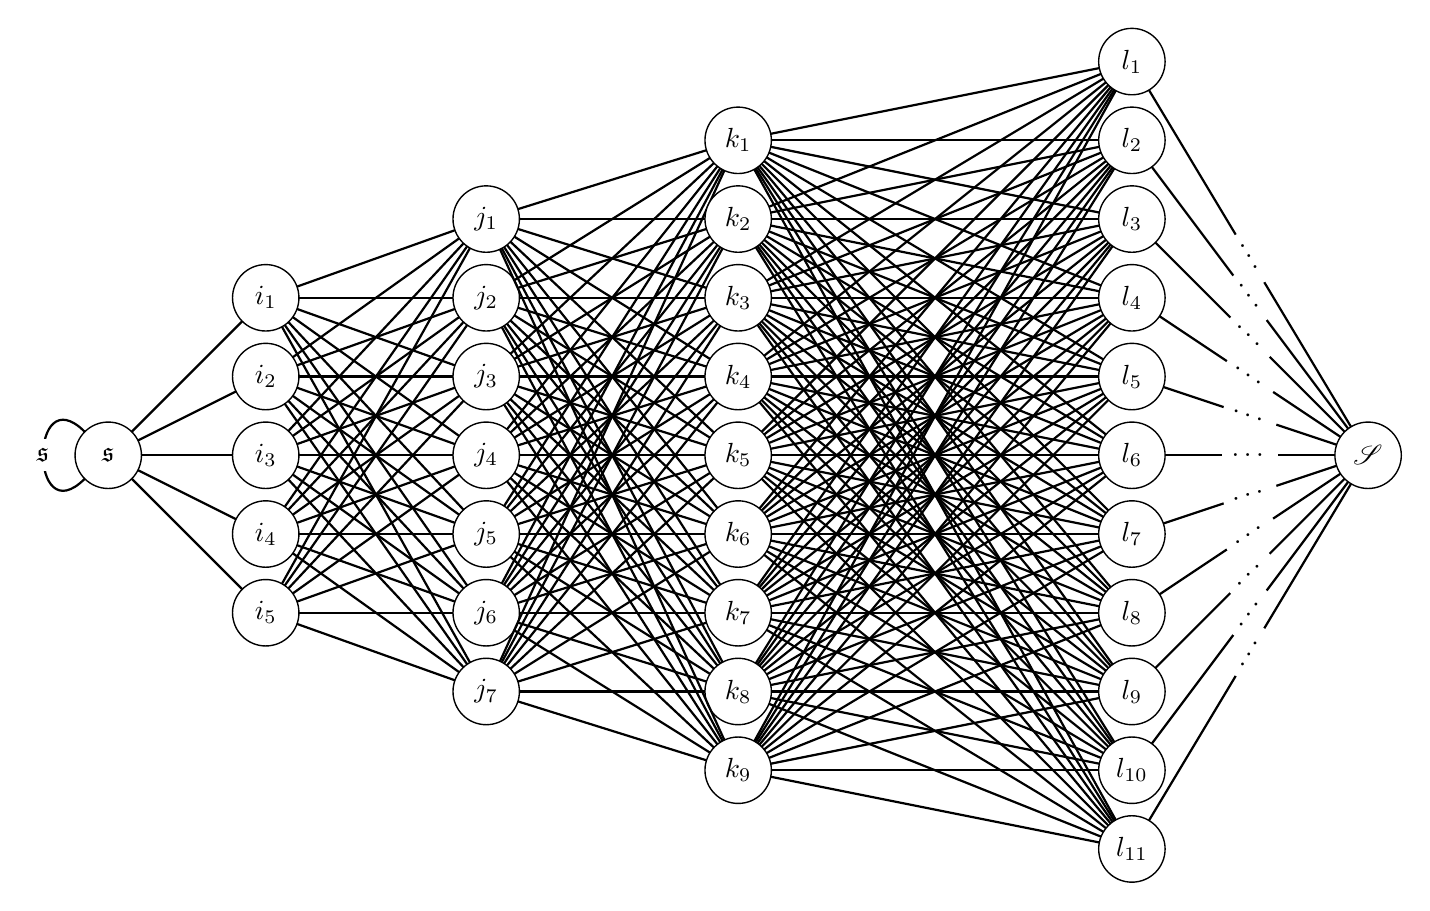
\begin{tikzpicture}
    \SetVertexMath
    \Vertex[x=-8, y=0,L=\mathfrak{s}]{s}
    \Loop[dist=1cm,label={$\mathfrak{s}$},style={thick,-}](s)
    \Vertex[x=8, y=0,L=\mathscr{S}]{S}

    \foreach \y [count=\n,evaluate={\m=int(6-\n)}] in {2,...,-2}
    {\Vertex[x=-6, y=\y, L=i_\n]{l1\m}
    \Edges(s, l1\m)}

    \foreach \y [count=\n,evaluate={\m=int(8-\n)}] in {3,...,-3}
    {\Vertex[x=-3.2, y=\y, L=j_\n]{l2\m}
        \foreach \k in {1,...,5}
    {\Edges(l1\k, l2\m)}}

    \foreach \y [count=\n,evaluate={\m=int(10-\n)}] in {4,...,-4}
    {\Vertex[x=0, y=\y, L=k_\n]{l3\m}
        \foreach \k in {1,...,7}
    {\Edges(l2\k,l3\m)}}

    \foreach \y [count=\n,evaluate={\m=int(12-\n)}] in {5,...,-5}
    {\Vertex[x=5, y=\y, L=l_{\n}]{l4\m}
        \draw[-,thick] (l4\m)--(S) node[midway,sloped,fill=white]{$\dots$};
        \foreach \k in {1,...,9}
    {\Edges(l3\k,l4\m)}}

\end{tikzpicture}
\end{document}
